% Options for packages loaded elsewhere
\PassOptionsToPackage{unicode}{hyperref}
\PassOptionsToPackage{hyphens}{url}
%
\documentclass[
]{article}
\usepackage{lmodern}
\usepackage{amsmath}
\usepackage{ifxetex,ifluatex}
\ifnum 0\ifxetex 1\fi\ifluatex 1\fi=0 % if pdftex
  \usepackage[T1]{fontenc}
  \usepackage[utf8]{inputenc}
  \usepackage{textcomp} % provide euro and other symbols
  \usepackage{amssymb}
\else % if luatex or xetex
  \usepackage{unicode-math}
  \defaultfontfeatures{Scale=MatchLowercase}
  \defaultfontfeatures[\rmfamily]{Ligatures=TeX,Scale=1}
\fi
% Use upquote if available, for straight quotes in verbatim environments
\IfFileExists{upquote.sty}{\usepackage{upquote}}{}
\IfFileExists{microtype.sty}{% use microtype if available
  \usepackage[]{microtype}
  \UseMicrotypeSet[protrusion]{basicmath} % disable protrusion for tt fonts
}{}
\makeatletter
\@ifundefined{KOMAClassName}{% if non-KOMA class
  \IfFileExists{parskip.sty}{%
    \usepackage{parskip}
  }{% else
    \setlength{\parindent}{0pt}
    \setlength{\parskip}{6pt plus 2pt minus 1pt}}
}{% if KOMA class
  \KOMAoptions{parskip=half}}
\makeatother
\usepackage{xcolor}
\IfFileExists{xurl.sty}{\usepackage{xurl}}{} % add URL line breaks if available
\IfFileExists{bookmark.sty}{\usepackage{bookmark}}{\usepackage{hyperref}}
\hypersetup{
  pdftitle={Techonology, Geography and Trade},
  pdfauthor={Jonathan Eaton \& Samuel Kortum},
  hidelinks,
  pdfcreator={LaTeX via pandoc}}
\urlstyle{same} % disable monospaced font for URLs
\usepackage{longtable,booktabs}
\usepackage{calc} % for calculating minipage widths
% Correct order of tables after \paragraph or \subparagraph
\usepackage{etoolbox}
\makeatletter
\patchcmd\longtable{\par}{\if@noskipsec\mbox{}\fi\par}{}{}
\makeatother
% Allow footnotes in longtable head/foot
\IfFileExists{footnotehyper.sty}{\usepackage{footnotehyper}}{\usepackage{footnote}}
\makesavenoteenv{longtable}
\usepackage{graphicx}
\makeatletter
\def\maxwidth{\ifdim\Gin@nat@width>\linewidth\linewidth\else\Gin@nat@width\fi}
\def\maxheight{\ifdim\Gin@nat@height>\textheight\textheight\else\Gin@nat@height\fi}
\makeatother
% Scale images if necessary, so that they will not overflow the page
% margins by default, and it is still possible to overwrite the defaults
% using explicit options in \includegraphics[width, height, ...]{}
\setkeys{Gin}{width=\maxwidth,height=\maxheight,keepaspectratio}
% Set default figure placement to htbp
\makeatletter
\def\fps@figure{htbp}
\makeatother
\setlength{\emergencystretch}{3em} % prevent overfull lines
\providecommand{\tightlist}{%
  \setlength{\itemsep}{0pt}\setlength{\parskip}{0pt}}
\setcounter{secnumdepth}{5}
\usepackage{ctex}

%\usepackage{xltxtra} % XeLaTeX的一些额外符号
% 设置中文字体
\setCJKmainfont[BoldFont={黑体},ItalicFont={楷体}]{新宋体}

\usepackage{amsthm,mathrsfs}
\usepackage{booktabs}
\usepackage{longtable}
\makeatletter
\def\thm@space@setup{%
  \thm@preskip=8pt plus 2pt minus 4pt
  \thm@postskip=\thm@preskip
}
\makeatother
\ifluatex
  \usepackage{selnolig}  % disable illegal ligatures
\fi
\usepackage[]{natbib}
\bibliographystyle{apalike}

\title{Techonology, Geography and Trade}
\author{Jonathan Eaton \& Samuel Kortum}
\date{Econometrica, 2002}

\begin{document}
\maketitle
\begin{abstract}
EK 模型是对李嘉图模型的扩展,它是一个包含现实地理特征的一般均衡模型。它为双边贸易提供了简单的结构方程,其中包含了反映绝对优势、比较优势(促进贸易)和地理障碍(抑制贸易)的参数。该文使用1990年19个 OECD 国家的制造业、价格和地理数据估计了这些参数,而后使用该模型讨论了各种问题,包括贸易利得、一国技术进步红利通过贸易扩散后的分布和关税削减的影响等。
\end{abstract}

{
\setcounter{tocdepth}{3}
\tableofcontents
}
\hypertarget{ux5f15ux8a00}{%
\section[引言]{\texorpdfstring{引言\footnote{在国际贸易领域,有两大经典模型:Melitz 模型和 EK 模型。EK 模型的核心,是一个包含地理特征的 \(n \times n \times 2\) 李嘉图一般均衡模型,即 \(n\) 个国家,\(n\) 中商品,2种要素。说它是李嘉图模型,因为它假定成本与产量无关,不存在规模经济,这就与新贸易理论拉开了距离。}}{引言}}\label{ux5f15ux8a00}}

\hypertarget{ux7406ux8bbaux521bux65b0}{%
\subsection{理论创新}\label{ux7406ux8bbaux521bux65b0}}

  国际贸易理论还没有掌握许多基本事实:

\begin{enumerate}
\def\labelenumi{(\arabic{enumi})}
\tightlist
\item
  随距离的增加,贸易急剧减少;\\
\item
  不同地区的物价不同,相距越远的地区之间差别越大;\\
\item
  要素报酬在各国之间相差甚远;\\
\item
  各国生产率在不同行业之间存在显著差异。
\end{enumerate}

  其中,(1) 和 (2) 表明地理在经济活动中起着重要作用。(3) 和 (4) 表明,各国都在使用不同的技术。很多文献分别处理了上述特征,但没有提供一个简单的框架以涵盖所有这些特点。

  我们提出了一个包含地理特征的李嘉图模型(一个基于技术差异的模型)。该模型综合了作用相反的两种因素:促进贸易的比较优势和抑制贸易的地理障碍(包括自然的和人为的)。这个广义的地理障碍反映了运输成本、关税和配额、延误\footnote{导致的不确定性。} 以及与远方交易对象谈判的不便\footnote{交易成本之一。} 等因素。

  该模型给出了双边贸易额与(1)购买力平价偏离和(2)技术和地理障碍之间关系的简单表达式。通过这两个关系,我们可以估计需要的参数,来解出模型的均衡,并观察该均衡对各种冲击的反应。

  本文的出发点是 \citet{DFS1977} 的两国连续统商品李嘉图模型。我们引入了表征技术异质性的概率公式,通过这个技巧,我们扩展出一个多国模型,并且这些国家受到地理障碍的分离。于是,我们有了一个将地理特征纳入一般均衡分析的框架,这个框架不仅是易处理的,而且是灵活、易扩展的。

  我们的模型的另一个特点是,它能够以一种简单的方式识别出中间品贸易的重要性。中间品贸易的大量存在使贸易对要素成本和地理障碍变得更加敏感。因此,通过对投入品成本的影响,地理位置在专业化\footnote{即贸易模式。} 的决定中起着重要作用。

\hypertarget{ux7814ux7a76ux7ed3ux8bba}{%
\subsection{研究结论}\label{ux7814ux7a76ux7ed3ux8bba}}

  我们使用1990年19个 OECD 国家的制造业双边贸易截面数据来估计我们的模型\footnote{制造业贸易在 OECD 国家之间的商品贸易中的占比达75\%以上。} 。参数对应于:(1)决定绝对优势的技术水平;(2)决定比较优势的技术异质程度;(3)地理障碍。我们采用不同策略来估计这些参数,使用了模型提供的多种结构方程,以及贸易流量、价格、地理和工资等多种数据。

  参数估计使我们能够量化模型的一般均衡,以便定量地讨论以下反事实情形:

\begin{enumerate}
\def\labelenumi{\arabic{enumi}.}
\item
  制造业贸易的利得。毫不奇怪,所有国家都从更自由的世界贸易中受益,但小国比大国获益更多。相对于转变为没有地理障碍的``零重力''世界的获益,制造业转向自给自足的世界的成本并不高\footnote{The cost of a move to autarky in manufactures is modest relative to the gains from a move to a ``zero gravity'' world with no geographic barriers.} 。这也说明,现实距离零地理障碍的极端情况相当遥远。
\item
  技术和地理如何决定专门化模式。随着地理障碍从自给自足水平下降,制造业转移到较大的国家,因为在那里中间投入品更便宜。但当地理障碍下降到一定程度时,进一步的下降将逆转这种模式,此时较小的国家也可以低价购买中间产品。这时,地理障碍的进一步下降对最大的国家不利,而对最小的国家有利。
\item
  一国技术进步红利通过贸易扩散后的分布。本国的技术进步几乎可以提高所有国家的福利。但是,只有临近本国且可以灵活缩减制造业规模的国家,其福利改善程度能够接近本国。
\item
  关税削减的影响。几乎每个国家都受益于多边贸易自由化,但若美国单方面降低关税,则会蒙受损失。根据区域内部劳动力流动情况,欧洲区域一体化有可能通过贸易转移(trade diversion)损害部分成员国,或通过贸易条件的恶化损害附近的非成员国。
\end{enumerate}

\hypertarget{ux7814ux7a76ux601dux8defux4e0eux65b9ux6cd5}{%
\subsection{研究思路与方法}\label{ux7814ux7a76ux601dux8defux4e0eux65b9ux6cd5}}

  除了少数例外,李嘉图模型很少作为贸易流量实证分析的基础,可能是因为它的标准公式掩盖了数据的许多一阶特征(如多个国家、多种产品、中间品贸易、地理障碍)。更活跃的前沿实证研究包括:(1)双边贸易流量的引力模型;(2)国际经济的 CGE(computable general equilibrium)模型;(3)用要素禀赋或 HOV(Heckscher-Ohlin-Vane) 模型解释贸易。

  我们的理论表明,双边贸易额呈现出一种类似于引力方程的结构,即贸易流量与距离和贸易伙伴国双边 GDP 有关。考虑到引力模型在解释数据方面的成功,我们模型的这一特征可以视为对引力模型的一个实证补充。但是,为了进行反事实研究,我们必须深入到引力方程的表象之下,揭示若干结构参数------这些参数决定了技术和地理在贸易中的作用。

  与 CGE 模型一样,我们在一般均衡框架下分析贸易流量,因此我们可以进行政策实验。但我们的设定比典型的 CGE 模型更简单。一方面,CGE 模型通常将每个国家的商品视为独特的,继而引入可分离偏好,如 Armington (1969)。与此相反,我们采用李嘉图方法来定义一组独立于国家的商品集,国家之间的专业化由比较优势决定。

  我们的方法与基于 HOV 模型的实证方法不太一样。HOV模型关注的是要素禀赋和专业化模式之间的关系。这项工作往往忽视了区位(通过忽视贸易成本)、技术(通过假设全球技术是相同的)和双边贸易额(因为模型给出对它们的预测)等因素。我们则使用了李嘉图式假设,即劳动力是唯一无法跨国流动的要素。原则上可以通过引入其他不可跨国流动的要素,来贯通这两种方法。

\hypertarget{ux5168ux6587ux7ed3ux6784}{%
\subsection{全文结构}\label{ux5168ux6587ux7ed3ux6784}}

  为了聚焦于模型最新奇的特性以及它们与数据之间的关系,我们以一种不太标准的顺序展开我们的分析。第二部分,首先将投入成本作为外生变量,在此条件下设定我们的贸易模型。它能够导出双边贸易流量与价格、地理障碍、技术水平和投入成本的关系。第三部分,我们对贸易-价格之间的关系进行了实证检验。第四部分,我们完善了模型,将投入成本作为内生变量。有了完整模型后,第五部分使用了几种不同的方法来估计模型参数。第六部分使用量化模型来探索上文列出的反事实情境。第七部分是结论。

\hypertarget{ux4e0dux5b8cux5907ux6a21ux578b}{%
\section[不完备模型]{\texorpdfstring{不完备模型\footnote{A Model of Technology, Prices, and Trade Flows. 半个一般均衡模型:将要素价格作为外生变量,仅考虑需求端。}}{不完备模型}}\label{ux4e0dux5b8cux5907ux6a21ux578b}}

  我们在 \citet{DFS1977} 的基础上构建模型,即由于技术水平的差异,各国对各种商品的生产效率不同。设 \(i\) 国生产 \(j\in[0,1]\) 产品的效率\footnote{该定义隐含了规模报酬不变的前提。} 为 \(z_i(j)\)。

  我们可以将两种主要生产要素划分为制造业劳动力和中间品(资本),生产所需``投入''就是这两种要素的混合。假设:(1)一国内部要素市场均衡时,制造业劳动和中间品的价格是处处相同的;(2)劳动和中间品在要素报酬中获取的份额恒定\footnote{这是一个 C-D 式生产函数的假设。} 。则一国制造业内部生产不同产品的单位投入\footnote{劳动与资本一定比例的混合。} 的成本是相同的。设 \(i\) 国单位投入的成本为 \(c_i\),于是 \(i\) 国生产一单位 \(j\) 产品的成本是 \({c_i}/{z_i(j)}\)。

  通过设定冰山型运输成本引入地理障碍。设 \(i\) 国向 \(n\) 国出口商品,\(n\) 国每接收1单位产品到岸,需要 \(i\) 国离岸出口 \(d_{ni}\) 单位产品,之间的差额被损耗掉。因此地理障碍意味着

\[
\left\{\begin{array}{c}{d_{i i}=1} \\ {d_{n i}>1, \forall n \neq i}\end{array}\right.
\]

  于是 \(i\) 国生产的 \(j\) 产品在 \(n\) 国的价格为

\begin{align}
p_{ni}(j)=(\frac {c_i}{z_i(j)})d_{ni} \label{eq:1}
\end{align}

  \(n\) 国则在全世界范围内挑选最低价,假定完全竞争\footnote{此处的完全竞争假设可以拓展为 Bertrand 竞争,参见 Bernard, Eaton, Jensen and Kortum (2000).} ,\(j\) 产品在 \(n\) 国的最终价格为:

\begin{align}
p_{n}(j)=\min \left\{p_{n i}(j) ; i=1, \cdots, N\right\}  \label{eq:2}
\end{align}

其中 \(N\) 为国家总数。

  此外,设各国的效用函数相同,为 CES 型:

\begin{align}
U=\left[\int_{0}^{1} Q(j)^{(\sigma-1) / \sigma} d j\right]^{\sigma /(\sigma-1)} \label{eq:3}
\end{align}

其中替代弹性 \(\sigma>0\)

\hypertarget{ux6280ux672f}{%
\subsection{技术}\label{ux6280ux672f}}

  设一国生产不同产品的效率服从该国特定的概率分布。则 \(i\) 国生产 \(j\) 产品的效率为一个随机变量 \(Z_i\),其分布函数为 \(F_i(z) \equiv Pr[Z_i \le z]\)\footnote{所有产品独立同分布,因而可以用一个分布函数代表。} 。根据大数定律,\(F_i(z)\) 也是\(i\) 国生产的所有产品中,效率低于 \(z\) 的产品的比例。

  由\eqref{eq:1}知,价格也是随机变量:\(i\) 国生产的所有产品在 \(n\) 国的价格服从同一个分布,都可以用随机变量 \(P_{n i}=c_{i} d_{n i} / Z_{i}\)来表示,从而 \(n\) 国最终消费的某种商品的价格为随机变量 \(P_{n}=\min \left\{P_{n i} ; i=1, \cdots, N\right\}\)。定义 \(i\) 国向 \(n\) 国提供某种商品的概率为 \(\pi_{n i}\)。要获得形式比较简单的价格分布函数和 \(\pi_{n i}\),需要对 \(F_i(z)\) 进行特殊设定。

  设 \(F_i(z)\) 服从 Fréchet 分布\footnote{又称 Type II extreme value distribution. 极值分布是从很多彼此独立的随机变量中挑出来的极大值(或者极小值)的概率分布。因 \(P_n\) 是取 \(N\) 个值中的极小值,故尝试了这种分布。} 且各国的分布相互独立:

\begin{align}
F_{i}(z)=e^{-T_{i} z^{-\theta}} \label{eq:4}
\end{align}

其中,\(T_i>0, \theta >1\)\footnote{\(\theta\) 参数对各国相同。} .

  该分布有性质:(1)\(Z_i\) 的几何均值为 \(e^{\gamma/\theta}T_i^{1/\theta}\)\footnote{\(\gamma\)为欧拉常数。} ,其对数的标准差为 \(\pi/(\theta \sqrt{6})\);(2)在 \(\theta\) 相同的前提下,\(T_i\) 反映各国的技术水平,该值越大,\(i\) 国企业以高效率生产的概率越大;(3)\(\theta\) 代表效率分布的离散程度,该值越小,分布越分散,各国之间克服地理障碍进行贸易的可能性越大。

\begin{figure}
\centering
\includegraphics{Figures/Frechet.png}
\caption{Fréchet 分布的概率密度函数}
\end{figure}

  如图1,为 \(Z_i\) 分布的概率密度函数,可以很直观地验证(2)和(3)两条性质。

\hypertarget{ux4ef7ux683c}{%
\subsection{价格}\label{ux4ef7ux683c}}

\hypertarget{ux4ef7ux683cux5206ux5e03}{%
\subsubsection{价格分布}\label{ux4ef7ux683cux5206ux5e03}}

  首先求 \(P_{ni}\) 的分布,定义其分布函数为

\[
G_{ni}(p) \equiv Pr[P_{ni} \le p]  
\]

  则有\footnote{\[
  \begin{aligned}
  G_{ni}(p) & \equiv Pr[P_{ni} \le p] \\  
  &= Pr[\frac {{c_i}d_{ni}}{Z_i} \le p]  = Pr[Z_i \geq \frac {{c_i}d_{ni}}{p}] \\ & = 1-Pr[Z_i \le \frac {{c_i}d_{ni}}{p}] = 1 - F_i(\frac {{c_i}d_{ni}}{p}) \\  
  &= 1 - e^{-T_{i} (\frac {{c_i}d_{ni}}{p})^{-\theta}} = 1-e^{-T_{i} ( {{c_i}d_{ni}})^{-\theta}p^{\theta}} 
  \end{aligned}
  \]} :

\begin{align}
G_{ni}(p) =1-e^{-T_{i} ( {{c_i}d_{ni}})^{-\theta}p^{\theta}}  \label{eq:5}
\end{align}

  这是 \(i\) 国出口到 \(n\) 国的某种产品价格小于等于 \(p\) 的概率,经过市场竞争,最终 \(n\) 国该种产品的价格小于等于 \(p\) 的概率为\footnote{\[
  \begin{aligned}
  G_n(p) &= Pr[P_n \le p] \\ &=Pr[ \min \left\{P_{n i} ; i=1, \cdots, N\right\} \le p] \\ &= 1 - Pr[ \min \left\{P_{n i} ; i=1, \cdots, N\right\} \geq p] \\ &= 1- Pr[ P_{n i}  \geq p; i=1, \cdots, N]\\ &=1-\prod_{i}Pr\left\{P_{ni}\geq p\right\} \\ &=1-\prod_{i}{(1-G_{ni}\left(p\right))}
  \end{aligned}
  \]}

\[
G_n(p) =1-\prod_{i}{(1-G_{ni}\left(p\right))}
\]

  将\eqref{eq:5}代入,得 \[G_n\left(p\right)=1-e^{-[\sum_{1}^{N}T_{i} ( {{c_i}d_{ni}})^{-\theta}]p^{\theta}} \]

  因此
\begin{align}
G_{n}(p)=1-e^{-\Phi_{n} p^{\theta}}  \label{eq:6}
\end{align}

  其中,定义价格参数
\begin{align}
\Phi_{n} = \sum_{1}^{N}T_{i} ( {{c_i}d_{ni}})^{-\theta}  \label{eq:7}
\end{align}

  价格参数 \(\Phi_n\) 非常重要,因为它包括了影响各国价格变量的3个因素:(1)技术水平;(2)要素成本;(3)地理障碍。

\hypertarget{phi_n-ux7684ux6027ux8d28}{%
\subsubsection{\texorpdfstring{\(\Phi_n\) 的性质}{\textbackslash Phi\_n 的性质}}\label{phi_n-ux7684ux6027ux8d28}}

\begin{enumerate}
\def\labelenumi{\arabic{enumi}.}
\tightlist
\item
  国家数量越多,或国家数量不变而 \(T_i\) 越大,都会使 \(\Phi_n\) 越大,从而 \(G_{n}(p)\) 越大,即价格的期望会越小。因此,通过国际贸易可以使得本国居民享受到更低的价格水平,就像本国技术提高了一样。\\
\item
  国际贸易的利得会受到要素成本和地理障碍的削弱。考虑两种极端情况:\\
  A. 零地理障碍,即 \(d_{n i} \equiv 1\) for all \(n\) and \(i\),此时 \(\Phi_{n} = \sum_{1}^{N}T_{i}{c_i}^{-\theta}\) 对于所有国家都一样,各国价格的分布完全相同------这就是概率版本的一价定律\\
  B. 自给自足,即 \(d_{n i} \rightarrow \infty\) for \(n \neq i\),此时 \(\Phi_{n} = T_{n}{c_n}^{-\theta}\),价格只受本国技术和要素成本影响。
\end{enumerate}

\hypertarget{ux4ef7ux683cux5206ux5e03ux7684ux4e09ux4e2aux6027ux8d28}{%
\subsubsection{价格分布的三个性质}\label{ux4ef7ux683cux5206ux5e03ux7684ux4e09ux4e2aux6027ux8d28}}

\begin{enumerate}
\def\labelenumi{\arabic{enumi}.}
\tightlist
\item
  \(n\) 国最终选择从 \(i\) 国购买某种产品的概率为\footnote{\[
    \begin{aligned}
    &\pi_{n i}=\operatorname{Pr}\left[P_{n i} \leq \min \left\{P_{n s}; s \neq i\right\}\right] \\ 
    &=\int\cdots\int_{\left[P_{n i} \leq \min \left\{P_{n s}; s \neq i\right\}\right]}{ \prod_{i=1}^{N} G_{n i}^{\prime} \left(p_{n i}\right) d p_{n 1} \cdots d p_{n n}} \\
    &={\int_{0}^{\infty} G_{n i}^{\prime}(p)\left[\prod_{s \neq i} \int_{p}^{\infty}G_{n s}^{\prime}\left(p_{n s}\right) d p_{n s}\right] d p}\\
    &={\int_{0}^{\infty} G_{n i}^{\prime}(p)\prod_{s \neq i} \left [1 - G_{n s}(p)\right] dp} \\
    &=\int_{0}^{\infty} \prod_{s \neq i}\left[1-G_{n s}(p)\right] d G_{ni}(p) \\ 
    &=\int_{0}^{\infty} \prod_{s \neq i}e^{ -T_{s}\left(c_{s} d_{n s}\right)^{-\theta} p^{\theta}} \cdot e^{ -T_{i}\left(c_{i} d_{n i}\right)^{-\theta} p^{\theta}} T_{i}\left(c_{i} d_{n i}\right)^{-\theta} d p^{\theta}\\
    & \text {      }=T_{i}\left(c_{i} d_{n i}\right)^{-\theta}\int_{0}^{\infty} e^{ -\Phi_n p^{\theta}}  d p^{\theta}\\
    &=\frac{T_{i}\left(c_{i} d_{n i}\right)^{-\theta}}{\Phi_{n}} 
    \end{aligned} 
    \]}
\end{enumerate}

\begin{align}
\pi_{n i}=\frac{T_{i}\left(c_{i} d_{n i}\right)^{-\theta}}{\Phi_{n}}  \label{eq:8}
\end{align}

  同时,\(\pi_{ni}\) 也是 \(\Phi_{n}\) 中 \(i\) 国的贡献比例。

  由大数定律知,\(n\) 国最终从 \(i\) 国购买的产品种类占 \(n\) 国消费全部产品种类的比例也是 \(\pi_{ni}\).

\begin{enumerate}
\def\labelenumi{\arabic{enumi}.}
\setcounter{enumi}{1}
\tightlist
\item
  \(n\) 国最终选择从 \(i\) 国购买某种产品,其价格的条件概率分布也是 \(G_{n}(p)\)。因此,来源国不影响 \(n\) 国\textbf{某一种}消费产品价格的概率分布。并且由大数定律知,最终 \(n\) 国从 \(i\) 国进口的所有产品的价格分布也是 \(G_{n}(p)\)。因此,来源国也不影响 \(n\) 国消费\textbf{多种}产品的价格分布。
\end{enumerate}

  如何理解这条性质呢?由\eqref{eq:11}知,技术水平高、投入成本低、到 \(n\) 国地理障碍少的国家,以所有产品计算,到达 \(n\) 国的商品到岸价格的均值会更低。但事实上,\(n\) 国只会购买该国生产最有效率的一部分产品。而对于缺乏竞争优势的国家,虽然以所有产品计算,到达 \(n\) 国的商品到岸价格的均值会高一些,但 \(n\) 国购买其产品更少,集中在其最有竞争力的商品上。最终,A source with a higher state of technology, lower input cost, or lower barriers exploits its advantage by selling a wider range of goods, exactly to the point at which the distribution of prices for what it sells in \(n\) is the same as \(n\)'s overall price distribution. 两国在 \(n\) 国出售商品的价格分布刚好一致。\footnote{比如,德国技术水平高,在许多产品中具有价格优势;西班牙技术水平低,具有价格优势的产品品种就比较少。但是,如果本国购买更多种类的德国产品,而只买很少数量的西班牙最有竞争力的产品,则最终对两国的平均购买价格可能是一样的。}

\begin{enumerate}
\def\labelenumi{\arabic{enumi}.}
\setcounter{enumi}{2}
\tightlist
\item
  在 \(\sigma < 1 + \theta\) 的前提下,CES 效用函数对应的价格指数\footnote{第四部分中可以推导,对于 CES 效用函数,满足 \(U=I/p\),\(I、p\) 分别为收入和价格指数。}
\end{enumerate}

\begin{align}
p_{n}=\gamma \Phi_{n}^{-1 / \theta}  \label{eq:9}
\end{align}

  其中 \(\gamma=\left[\Gamma\left(\frac{\theta+1-\sigma}{\theta}\right)\right]^{1 /(1-\sigma)}\),因各国的 \(\Phi_{n}\) 受到地理障碍的影响而不同,故各国的价格指数不同。因此,地理障碍这个因素使各国价格偏离一价定律,且越远离其他国家的国家,其价格指数越大。

\hypertarget{ux8d38ux6613ux6d41ux91cfux548cux5f15ux529b}{%
\subsection{贸易流量和引力}\label{ux8d38ux6613ux6d41ux91cfux548cux5f15ux529b}}

  由上一节价格分布的性质2知,\(n\) 国消费的每种产品的价格分布与来源地无关,均服从 \(G_n(p)\) 分布。在连续统商品的假设下,\(n\) 国从每个国家都购买了无穷多种商品,则 \(n\) 国从每个国家购买的商品的平均价格应为 \(G_n(p)\) 这个分布所对应的期望,是相同的。因此 \(n\) 国从一个国家的进口支出与从该国进口的商品数量成正比。

  又因为效用函数是对称的,在所有商品价格服从同一分布的前提下,其消费数量也服从同一分布。故由大数定律,从一国进口商品的数量与进口商品的种类成正比。因此,\(n\) 国从 \(i\) 国进口支出占 \(n\) 国总支出的比例,就等于 \(n\) 国从 \(i\) 国进口商品种类占所有消费商品种类的比例 \(\pi_{ni}\),即:

\begin{align}
\frac{X_{n i}}{X_{n}}=\pi_{ni}=\frac{T_{i}\left(c_{i} d_{n i}\right)^{-\theta}}{\Phi_{n}}=\frac{T_{i}\left(c_{i} d_{n i}\right)^{-\theta}}{\sum_{k=1}^{N} T_{k}\left(c_{k} d_{n k}\right)^{-\theta}} \label{eq:10}
\end{align}

其中,\(X_{n}\) 为 \(n\) 国总支出,\(X_{n i}\) 为 \(n\) 国对 \(i\) 国的总进口额。

  \(i\) 作为出口国,其总销售额为:

\[
Q_{i}=\sum_{m=1}^{N} X_{m i}=T_{i} c_{i}^{-\theta} \sum_{m=1}^{N} \frac{d_{m i}^{-\theta} X_{m}}{\Phi_{m}}
\]

  由此可求出 \(T_{i} c_{i}^{-\theta}\) 的表达式,将其代入\eqref{eq:10}并结合\eqref{eq:9}得到

\begin{align}
X_{n i}=\frac{\left(\frac{d_{n i}}{p_{n}}\right)^{-\theta} X_{n}}{\sum_{m=1}^{N}\left(\frac{d_{m i}}{p_{m}}\right)^{-\theta} X_{m}} Q_{i} \label{eq:11}
\end{align}

  \eqref{eq:11}是一个标准的{引力方程}。它具有以下性质:(1)双边贸易额对 \(X_n\) 和 \(Q_i\) 的弹性为1\footnote{前提是 \(N\) 充分大。} 。(2)地理障碍 \(d_{ni}\) 被进口国的价格指数 \(p_n\) 缩减。给定 \(i\) 国的总出口额 \(Q_i\),可以将 \({\left({d_{n i}}/{p_{n}}\right)^{-\theta} X_{n}}\) 视为 \(n\) 国对于 \(i\) 国的市场份额,从而\eqref{eq:11}右边的分母就是 \(i\) 国眼中的全球市场。\(p_n\) 的下降与地理障碍 \(d_{ni}\) 的上升具有相同的作用,即阻碍 \(i\) 国进入 \(n\) 国\footnote{地理障碍越大,进口国本国物价越便宜,出口国的商品越不容易进来。} 。

\hypertarget{ux8d38ux6613ux5730ux7406ux548cux4ef7ux683cux521dux63a2}{%
\section{贸易、地理和价格初探}\label{ux8d38ux6613ux5730ux7406ux548cux4ef7ux683cux521dux63a2}}

\hypertarget{ux6807ux51c6ux5316ux7684ux8fdbux53e3ux4efdux989d}{%
\subsection[标准化的进口份额]{\texorpdfstring{标准化的进口份额\footnote{Normalized Import Share.}}{标准化的进口份额}}\label{ux6807ux51c6ux5316ux7684ux8fdbux53e3ux4efdux989d}}

  在\eqref{eq:10}中取 \(n\) 为 \(i\),然后再相除,得到

\begin{align}
\frac{X_{n i} / X_{n}}{X_{i i} / X_{i}}=\frac{\Phi_{i}}{\Phi_{n}} d_{n i}^{-\theta}=\left(\frac{p_{i} d_{n i}}{p_{n}}\right)^{-\theta} \label{eq:12}
\end{align}

  \eqref{eq:12}左边为 \(i\) 国在 \(n\) 国支出中的占比除以 \(i\) 国在 \(i\) 国支出中的占比,称为标准化的 \(n\) 国进口中来源于 \(i\) 国的份额(\(n\)'s normalized import share from \(i\))。

\begin{itemize}
\tightlist
\item
  这个值不会超过1。因为,\(\frac{X_{n i} / X_{n}}{X_{i i} / X_{i}}>1 \Rightarrow \frac{p_{i} d_{n i}}{p_{n}}<1\),若该式成立,\(n\) 国消费的所有产品都可以从 \(i\) 国进口以节省开支(a purchaser in country \(n\) can always buy all her goods in \(i\) at a price index \(p_{i} d_{n i}\)),这与 \(n\) 国选择了最低价格是矛盾的。\\
\item
  \(i\)'s normalized share in \(n\) 的性质

  \begin{itemize}
  \tightlist
  \item
    \(p_i/p_n \uparrow\) 或 \(d_{ni} \uparrow\) 使标准化支出份额下降\\
  \item
    \(\theta \uparrow\) 反映比较优势减弱,可贸易范围减少,使标准化支出份额下降。
  \end{itemize}
\end{itemize}

\hypertarget{ux4f30ux8ba1-theta}{%
\subsection{\texorpdfstring{估计 \(\theta\)}{估计 \textbackslash theta}}\label{ux4f30ux8ba1-theta}}

\begin{enumerate}
\def\labelenumi{\arabic{enumi}.}
\tightlist
\item
  使用制造业进出口数据,毕竟是可贸易性相对比较强的产品\\
\item
  取50种产品在样本国家中的零售数据,并进行对数化处理:\(r_{n i}(j)=\ln p_{n}(j)-\ln p_{i}(j)\)。对这 50 种产品的 \(-r_{n i}(j)\) 取平均值,作为 \(p_i/p_n\)\\
\item
  用第二大\footnote{避免异常值的影响。} 的 \(r_{n i}(j)\) 代表 \(\ln d_{ni}\)。因为按照本文的理论,\(n\) 国从 \(i\) 国进口的产品 \(j\) 满足 \(r_{n i}(j)=\ln d_{ni}\),\(n\) 国从第三国进口的产品 \(k\) 的价格比从 \(i\) 国进口更便宜,因此有 \(r_{n i}(k)<\ln d_{ni}\),故选取最大的 \(r_{n i}\) 作为 \(\ln d_{ni}\) 的代理变量(proxy)。
\item
  最终,令
\end{enumerate}

\begin{align}
D_{n i} \equiv \max 2_{j}\left\{r_{n i}(j)\right\}-\frac{1}{50}\sum_{j=1}^{50}\left[r_{n i}(j)\right] \label{eq:13}
\end{align}

  作为 \(\ln ({p_{i} d_{n i}}/{p_{n}})\) 的代理变量(price measure)。\(exp(D_{n i})\) 表示一个 \(n\) 国人若全部从 \(i\) 国购买商品,比在本国购买会贵多少(a buyer who insisted on purchasing everything from source \(i\), relative to the actual price index in \(n\), the price index for a buyer purchasing each goodfrom the cheapest source)

\begin{center}\includegraphics[width=0.8\linewidth]{Figures/Table2} \end{center}

  有了贸易流量和 \({p_{i} d_{n i}}/{p_{n}}\) 的数据,便可以利用\eqref{eq:12}估计 \(\theta\),估计结果如图2:

\begin{center}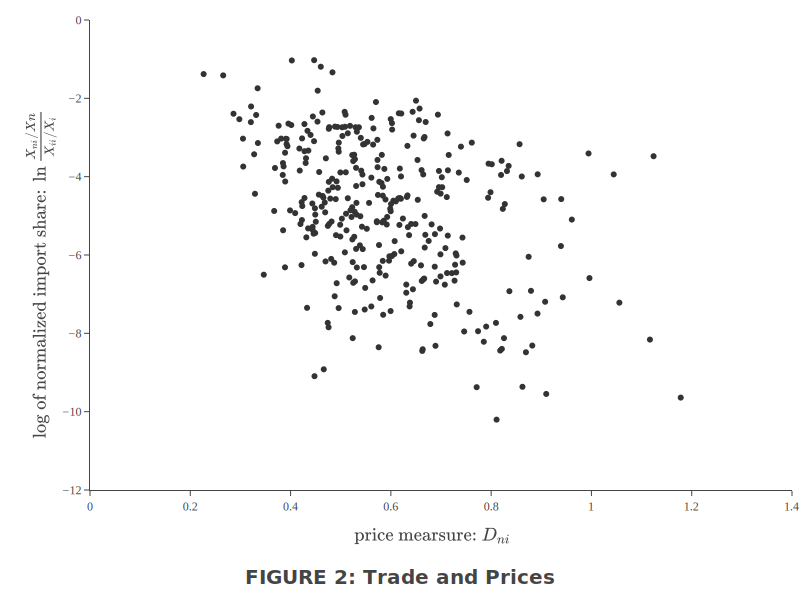
\includegraphics[width=0.8\linewidth]{Figures/Figure2} \end{center}

  利用 \(D_{ni}\) 代理变量估计 \(\theta\) 的值约为8.28.

\hypertarget{ux5b8cux5907ux6a21ux578b}{%
\section[完备模型]{\texorpdfstring{完备模型\footnote{Equilibrium Input Costs. 完整的一般均衡模型,将要素价格作为内生变量。}}{完备模型}}\label{ux5b8cux5907ux6a21ux578b}}

  前面讨论的双边贸易流与价格和地理的关系都建立在要素价格外生的前提下。本部门将要素价格内生化。我们将首先在劳动力价格给定条件下讨论中间产品价格的决定,最后再对劳动力价格建立一般均衡模型。

\hypertarget{ux751fux4ea7}{%
\subsection{生产}\label{ux751fux4ea7}}

\hypertarget{ux751fux4ea7ux51fdux6570ux4e0eux4e24ux9636ux6bb5ux6700ux4f18ux5316}{%
\subsubsection{生产函数与两阶段最优化}\label{ux751fux4ea7ux51fdux6570ux4e0eux4e24ux9636ux6bb5ux6700ux4f18ux5316}}

  假设生产要使用劳动和中间投入品,且生产函数为适用两阶段最优化的 D-S Lite 型,见 \citet{DS1977} ,即:(1)总成本中劳动 \(L\) 所占份额 \(\beta\) 保持不变;(2)中间品投入 \(Q(j)\) 以 CES 方式组织起来。具体形式如下\footnote{各国生产函数只有表示效率的 \(z_i(j)\) 这个唯一的区别。} :

\[
y_{i}(j)=\frac{z_{i}(j)}{\beta^{\beta}(1-\beta)^{1-\beta}} L^{\beta}\left\{\left[\int_{0}^{1} Q(j)^{\frac{\sigma-1}{\sigma}} d j\right]^{\frac{\sigma}{\sigma-1}}\right\}^{1-\beta}
\]

  则成本最小化问题为

\[
\left\{\begin{array}{c}
{\min_{L, Q} w_{i}L + \int_{0}^{1} P_{i}(j)Q(j) d j} \\ {\text { s.t. }\frac{z_{i}(j)}{\beta^{\beta}(1-\beta)^{1-\beta}} L^{\beta}\left\{\left[\int_{0}^{1} Q(j)^{\frac{\sigma-1}{\sigma}} d j\right]^{\frac{\sigma}{\sigma-1}}\right\}^{1-\beta}=y_{i}(j)}
\end{array}\right.
\]

  为便于求解,将其对偶化为产量最大化问题,并进行三个换元

\begin{itemize}
\tightlist
\item
  令效率指数 \(k_{i}(j)=\frac{z_{i}(j)}{\beta^{\beta}(1-\beta)^{1-\beta}}\)
\item
  令中间品数量指数 \(K=\left[\int_{0}^{1} Q(j)^{\frac{\sigma-1}{\sigma}} d j\right]^{\frac{\sigma}{\sigma-1}}\)
\item
  令中间品价格指数 \(p_{i}(j)=\left[\int_{0}^{1} P_{i}(j)^{1-\sigma} d j\right]^{\frac{1}{1-\sigma}}\),可以证明其为 \(\gamma \Phi_{i}^{-1 / \theta}\),与产品无关,故可以统一写为 \(p_{i}\). 且有 \(p_{i}K=\int_{0}^{1} P_{i}(j)Q(j) d j\)
\end{itemize}

  于是最优化问题变为

\[
\left\{\begin{array}{c}
{\max_{L, K} y_{i}(j)=k_{i}(j)L^{\beta}K^{1-\beta}} \\ {\text { s.t. } w_{i}L + p_{i}K = C}
\end{array}\right.
\]

  易知 \(L^*=\beta C/w_i, K^*=(1-\beta)C/p_i\),因此 \(i\) 国生产 \(j\) 产品的单价为

\[\frac{C}{y_{i}(j)}=\frac{w_{i}^{\beta}p_{i}^{1-\beta}}{z_{i}(j)}\]

  而由\eqref{eq:1}知该价格为 \(c(i)/{z_{i}(j)}\),故有

\begin{align}
c(i)=w_{i}^{\beta}p_{i}^{1-\beta} \label{eq:14}
\end{align}

  可见,生产产品 \(j\) 的单价与效率 \(z_{i}(j)\) 成反比,与 \(c(i)\) 则成正比,正是在这个意义上,我们称 \(c(i)\) 为 \(i\) 国单位投入的成本。

\hypertarget{ux798fux5229ux5b9eux9645ux5de5ux8d44}{%
\subsubsection{福利(实际工资)}\label{ux798fux5229ux5b9eux9645ux5de5ux8d44}}

  由\eqref{eq:8}得 \(\pi_{ii}=\frac{T_{i}c_{i}^{-\theta}}{\Phi_{i}}\),再利用\eqref{eq:9}将 \(\Phi_{i}\) 换为 \(p_{i}\),则有 \(\pi_{ii}=\frac{T_{i}p_{i}^{\theta}}{c_{i}^{\theta}\gamma^{\theta}}\),故

\[\frac{c_i}{p_i}=\frac{1}{\gamma}\left(\frac{T_i}{\pi_{ii}}\right)^{\frac{1}{\theta}}\]

  结合\eqref{eq:14}可得

\begin{align}
\frac{w_i}{p_i}=\left(\frac{c_i}{p_{i}}\right)^{\frac{1}{\beta}}=\gamma^{-1/\beta}\left(\frac{T_i}{\pi_{ii}}\right)^{\frac{1}{\beta\theta}} \label{eq:15}
\end{align}

  由于 \(\pi_{ii}\) 是 \(i\) 国最终支出中来源于本国产品的比例,显然,从自给自足到开放经济,\(\pi_{ii} \downarrow\),从而实际工资上升,福利改善。

\hypertarget{ux4e2dux95f4ux4ea7ux54c1ux4ef7ux683c}{%
\subsection{中间产品价格}\label{ux4e2dux95f4ux4ea7ux54c1ux4ef7ux683c}}

  将\eqref{eq:14}代入\eqref{eq:7}再代入\eqref{eq:9}中得:

\begin{align}
p_{n}=\gamma\left[\sum_{i=1}^{N} T_{i}\left(d_{n i} w_{i}^{\beta} p_{i}^{1-\beta}\right)^{-\theta}\right]^{-1 / \theta} \label{eq:16}
\end{align}

  将工资向量作为外生变量,则理论上,解这个 \(N\) 元方程组,就可以解出 \(p\) 向量。

  把\eqref{eq:14}和\eqref{eq:9}代入\eqref{eq:10},可得

\begin{align}
\frac{X_{n i}}{X_{n}}=\pi_{n i}=T_{i}\left(\frac{\gamma d_{n i} w_{i}^{\beta} p_{i}^{1-\beta}}{p_{n}}\right)^{-\theta} \label{eq:17}
\end{align}

  解出价格向量后,由\eqref{eq:17}可以求得进口来源份额。

\hypertarget{ux8981ux7d20ux4ef7ux683c}{%
\subsection{要素价格}\label{ux8981ux7d20ux4ef7ux683c}}

  设经济有两个部门:制造业部门和非制造业部门。后者的产品不可进行国际贸易,也不以制造业产品为中间投入\footnote{可以将其大致理解为 local service} 。

  \(i\) 国制造业部门的劳动力收入是 \(i\) 国制造业总出口(包括在国内的销售)中的劳动力收入份额。所以有

\begin{align}
w_{i} L_{i}=\beta \sum_{n=1}^{N} \pi_{n i} X_{n} \label{eq:18}
\end{align}

其中,\(L_i\) 为 \(i\) 国制造业工人数量,\(X_n\) 为 \(n\) 国对制造业产品的总支出。

  定义 \(n\) 国对所有最终产品的支出为 \(Y_n\),其中花费在制造业产品上的占比为固定值 \(\alpha\),则

\begin{align}
X_{n}=\frac{1-\beta}{\beta} w_{n} L_{n}+\alpha Y_{n} \label{eq:19}
\end{align}

其中,第一项为 \(n\) 国制造业生产(\(w_{n}L_{n}/\beta\))对中间产品的支出,第二项为 \(n\) 国所有人口对制造业最终产品的支出。

  从另一个角度看, \(Y_n\) 也是总收入,包括制造业劳动力的收入 \(Y_n^M\) 和非制造业劳动力的收入 \(Y_n^O\).

\hypertarget{ux6781ux7aefux60c5ux51b5}{%
\subsubsection{极端情况}\label{ux6781ux7aefux60c5ux51b5}}

  为了便于确立一般均衡框架,考虑两种极端情况,并对非制造业作出严格的假设:

\begin{enumerate}
\def\labelenumi{\arabic{enumi}.}
\item
  情境一:劳动力可在两部门间自由流动,且工资 \(w_i\) 由非制造业的生产率外生给定\footnote{达到刘易斯拐点之前的发展中大国?} ,劳动力禀赋也是外生的,从而总收入 \(Y_n\) 是外生给定的。且由\eqref{eq:16}可解出 \(p_i\)。结合\eqref{eq:18}和\eqref{eq:19}可得
  \begin{align}
  w_{i} L_{i}=\sum_{n=1}^{N} \pi_{n i}\left[(1-\beta) w_{n} L_{n}+\alpha \beta Y_{n}\right] \label{eq:20}
  \end{align}
  将\eqref{eq:17}中的 \(\pi_{ni}\)代入上式,得到 \(N\) 个方程,再将解出的 \(p_i\) 代入,可解得 \(L_{i}\) 向量。\(i\) 国制造业就业规模 \(L_{i}\) 受到 \(T_i\) 的影响,因此在劳动力自由流动的情况下,\(T_i\) 还反映了制造业相对于非制造业的比较优势。
\item
  情境二:劳动力不能跨部门流动,各国制造业就业规模 \(L_{i}\) 外生,且非制造业收入 \(Y_n^O\) 外生(同样有非制造业的工资水平外生)。结合\eqref{eq:18}和\eqref{eq:19}可得
  \begin{align}
  w_{i} L_{i}=\sum_{n=1}^{N} \pi_{n i}\left[(1-\beta+\alpha \beta) w_{n} L_{n}+\alpha \beta Y_{n}^{O}\right] \label{eq:21}
  \end{align}
  将\eqref{eq:17}中的 \(\pi_{ni}\)代入上式,得到 \(N\) 个方程,再结合\eqref{eq:16}的 \(N\) 个方程,可解出 \(p_i\) 与 \(w_{i}\) 向量。在劳动力不能自由流动的情况下,技术参数 \(T_i\) 影响制造业工资和价格水平。
\end{enumerate}

\hypertarget{ux96f6ux5f15ux529bux548cux81eaux7ed9ux81eaux8db3}{%
\subsection{零引力和自给自足}\label{ux96f6ux5f15ux529bux548cux81eaux7ed9ux81eaux8db3}}

  按照上述两种极端情况,一般均衡模型必然有解,但很难求出解析解,继续讨论两种特殊情况:

\hypertarget{ux5730ux7406ux969cux788dux6d88ux5931}{%
\subsubsection{地理障碍消失}\label{ux5730ux7406ux969cux788dux6d88ux5931}}

  此时 \(d_{ni}=1\),化简\eqref{eq:16}发现 \(p_i\) 的表达式对 \(i=1,2,\cdots,N\) 是相同的,从而各国价格水平一致,一阶定律成立。进一步化简\eqref{eq:17}得

\[\pi_{n i}=T_{i}\left(\frac{\gamma d_{n i} w_{i}^{\beta} p_{i}^{1-\beta}}{p_{n}}\right)^{-\theta}=T_{i}\left(\gamma w_{i}^{\beta} p_{i}^{-\beta}\right)^{-\theta}\]

  从而由\eqref{eq:18}得

\[
w_{i} L_{i}=\beta \sum_{n=1}^{N} \pi_{n i} X_{n}=\beta T_{i}\left(\gamma w_{i}^{\beta} p_{i}^{-\beta}\right)^{-\theta} \sum_{n=1}^{N} X_{n}
\]

  因此
\[\frac{w_{i} L_{i}}{w_{N} L_{N}}=\frac{T_{i}\left(w_{i}^{\beta} p_{i}^{-\beta}\right)^{-\theta}}{T_{N}\left(w_{N}^{\beta} p_{N}^{-\beta}\right)^{-\theta}}=\frac{T_{i}\left(w_{i}^{\beta}\right)^{-\theta}}{T_{N}\left(w_{N}^{\beta}\right)^{-\theta}}\]

  故有
\begin{align}
\frac{w_{i}}{w_{N}}=\frac{w_i/p_i}{w_n/p_n}=\left[\frac{T_{i} / L_{i}}{T_{N} / L_{N}}\right]^{\frac{1}{1+\theta \beta}} \label{eq:22}
\end{align}

  和
\[\frac{L_n}{L_i}=\left(\frac{w_i}{w_n}\right)^{1+\theta\beta}\frac{T_n}{T_i}\]

  讨论其含义:

\begin{enumerate}
\def\labelenumi{\arabic{enumi}.}
\tightlist
\item
  劳动力可在两部门间自由流动时,工资外生,技术水平 \(T_n\) 相对于工资越高,\(n\) 国制造业劳动力相对越多(越专业化于制造业)。\\
\item
  劳动力不能跨部门流动时,制造业劳动力数量外生,此时相对工资取决于人均技术水平之比。这个比值越大,工资水平越高。
\item
  给定技术水平,一国制造业劳动力的增加将导致制造业工资的下降。
\end{enumerate}

  进一步假定经济只有制造业一个部门,则由\eqref{eq:16}得

\[
\begin{array}{l}{p_{n}=\gamma\left[\sum_{i=1}^{N} T_{i}\left(w_{i}^{\beta} p_{i}^{1-\beta} d_{n i}\right)^{-\theta}\right]^{-\frac{1}{\theta}}} \\ {\Rightarrow p=p_{i}=\gamma^{\frac{1}{\beta}}\left[\sum_{i=1}^{N} T_{i}\left(w_{i}^{\beta}\right)^{-\theta}\right]^{-\frac{1}{\theta \beta}} \quad\left(d_{n i}=1, p_{n}=p_{i}\right)}\end{array}
\]

  结合\eqref{eq:22}有实际工资

\[
\begin{array}{l}{W_{i}=\frac{w_{i}}{p}=\frac{w_{i}}{\gamma^{\frac{1}{\beta}}}\left[\sum_{k=1}^{N} T_{k}\left(w_{k}^{\beta}\right)^{-\theta}\right]^{\frac{1}{\theta \beta}}} \\ {=\frac{1}{\gamma^{\frac{1}{\beta}}}\left[\sum_{k=1}^{N} T_{k}\left(\frac{w_{i}}{w_{k}}\right)^{\beta \theta}\right]^{\frac{1}{\theta \beta}}} \\ {=\frac{1}{\gamma^{\frac{1}{\beta}}}\left[\sum_{k=1}^{N} T_{k}\left(\frac{T_{i} / L_{i}}{T_{k} / L_{k}}\right)^{\frac{\beta \theta}{1+\theta \beta}}\right]^{\frac{1}{\theta \beta}}}\end{array}
\]

  因此

\begin{align}
W_{i}=\gamma^{-\frac{1}{\beta}} T_{i}^{\frac{1}{1+\theta \beta}}\left[\sum_{k=1}^{N} T_{k}^{\frac{1}{1+\theta \beta}}\left(L_{k} / L_{i}\right)^{\frac{\beta \theta}{1+\theta \beta}}\right]^{\frac{1}{\theta \beta}} \label{eq:23}
\end{align}

  可见,任何国家的技术水平 \(T_k\) 提高,\(i\) 国的福利都会上升。\(i\) 国自身技术水平提高时,会带来额外收益,因为它将提高本国对外国的相对工资。\(i\) 国从 \(k\) 国技术水平 \(T_k\) 的提高中获得的收益大小取决于 \(k\) 国相对于 \(i\) 国的劳动力数量。如果技术进步来源国 \(k\) 国的劳动力数量比较少,\(w_k\) 上升得更多,减少了 \(k\) 国技术水平提高给其他国家带来的利得。

\hypertarget{ux81eaux7ed9ux81eaux8db3}{%
\subsubsection{自给自足}\label{ux81eaux7ed9ux81eaux8db3}}

  此时 \(d_{n i} \rightarrow \infty, \forall n \neq i\). 在\eqref{eq:15}中取 \(\pi_{ii}=1\),得

\begin{align}
\quad W_{i}=\gamma^{-1 / \beta} T_{i}^{1 / \theta \beta}=\gamma^{-\frac{1}{\beta}} T_{i}^{\frac{1}{1+\theta \beta}}\left(T_{i}^{\frac{1}{1+\theta \beta}}\right)^{\frac{1}{\theta \beta}} \label{eq:24}
\end{align}

  \eqref{eq:23}比\eqref{eq:24}大\footnote{后者只是前者连加式中的一项。} ,因此每个国家均从贸易中受益了。

\hypertarget{ux4f30ux8ba1ux8d38ux6613ux65b9ux7a0b}{%
\section{估计贸易方程}\label{ux4f30ux8ba1ux8d38ux6613ux65b9ux7a0b}}

  式\eqref{eq:16}、\eqref{eq:17}再加上\eqref{eq:20}或\eqref{eq:21}构成了一个一般均衡。这些方程决定了价格水平、贸易份额、制造业工资(劳动力不可跨部门流动)或者制造业就业(劳动力可以跨部门流动)。这一部分我们主要估计一般均衡模型的参数,并在第六部分进行反事实分析。

\hypertarget{ux4f30ux8ba1ux6765ux6e90ux5730ux6548ux5e94}{%
\subsection{估计来源地效应}\label{ux4f30ux8ba1ux6765ux6e90ux5730ux6548ux5e94}}

  \eqref{eq:17}将双边贸易量同两国各自的特质和地理信息联系了起来,对该式的估计使我们可以了解技术水平与地理障碍。

  使用进口国的国内开支对\eqref{eq:17}的双边贸易数据进行标准化,根据\eqref{eq:17},令 \(\frac{X_{ni}}{X_n}\) 与 \(\frac{X_{nn}}{X_n}\) 两式相除可得

\begin{align}
\frac{X_{n i}}{X_{n n}}=\frac{\pi_{n i}}{\pi_{n n}}=\frac{T_{i}}{T_{n}}\left(\frac{w_{i}}{w_{n}}\right)^{-\theta \beta}\left(\frac{p_{i}}{p_{n}}\right)^{-\theta(1-\beta)} d_{n i}^{-\theta} \label{eq:25}
\end{align}

  同样由\eqref{eq:17}可得

\[
\begin{aligned}
\frac{X_{n n}}{X_{n}}&=\pi_{n n}=T_{n}\gamma^{-\theta}\left(\frac{w_{n}}{p_{n}}\right)^{-\beta\theta } \\
\frac{X_{i i}}{X_{i}}&=\pi_{i i}=T_{i}\gamma^{-\theta}\left(\frac{w_{i}}{p_{i}}\right)^{-\beta\theta } 
\end{aligned}
\]

  两式相除得

\[
\frac{p_{i}}{p_{n}}=\frac{w_{i}}{w_{n}}\left(\frac{T_{i}}{T_{n}}\right)^{-1 / \theta \beta}\left(\frac{X_{i} / X_{i i}}{X_{n} / X_{n n}}\right)^{-1 / \theta \beta}
\]

  代入\eqref{eq:25}消掉 \({p_i}/{p_n}\) 得到

\[
\ln \frac{X_{n i}}{X_{n n}}-\frac{1-\beta}{\beta}\ln \frac{X_{i} / X_{i i}}{X_{n} / X_{n n}}=-\theta \ln d_{n i}+\frac{1}{\beta} \ln \frac{T_{i}}{T_{n}}-\theta \ln \frac{w_{i}}{w_{n}}
\]

  为了化简该式,定义 \(\ln X_{n i}^{\prime} \equiv \ln X_{ni}-[(1-\beta)/\beta] \ln (X_i/X_{ii})\),则有

\begin{align}
\ln \frac{X_{n i}^{\prime}}{X_{n n}^{\prime}}=-\theta \ln d_{n i}+\frac{1}{\beta} \ln \frac{T_{i}}{T_{n}}-\theta \ln \frac{w_{i}}{w_{n}} \label{eq:26}
\end{align}

  进一步化简,定义

\begin{align}
S_i \equiv \frac{1}{\beta} \ln T_i - \theta \ln w_i \label{eq:27}
\end{align}

则有

\begin{align}
\ln \frac{X_{n i}^{\prime}}{X_{n n}^{\prime}}=-\theta \ln d_{n i}+S_i-S_n \label{eq:28}
\end{align}

  其中,\(S_i\) 可以视为 \(i\) 国的竞争力\footnote{与技术正相关,与工资负相关。} ,\eqref{eq:28}是我们要估计的基本方程\footnote{经过标准化后,该式允许我们忽略样本内国家与样本外国家的贸易。} 。

\begin{enumerate}
\def\labelenumi{\arabic{enumi}.}
\tightlist
\item
  利用双边贸易数据,并取 \(\beta\) 的平均值0.21,\eqref{eq:28}的左边便是确定的了。\\
\item
  至于等式右边,我们将每一个国家的竞争优势视为一个虚拟变量,\(S_i\) 就是来源国虚拟变量的系数(coefficients on source-country dummy)。\\
\item
  最后则是地理壁垒 \(d_{ni}\),根据引力方程的文献,我们用一系列代理变量来表示它,包括距离、语言和贸易协定。对于所有的 \(i \neq n\),建立回归模型:
\end{enumerate}

\begin{align}
\ln d_{n i}=d_{k}+b+l+e_{h}+m_{n}+\delta_{n i} \label{eq:29}
\end{align}

  其中 \(d_k\) 表征六档离散距离的效应,\(b\) 表征共同边界,\(l\) 表征共同语言,\(e_h\) 表征是否共同存在于一个区域贸易协定,\(m_n\) 表征目的地国效应\footnote{衡量目的地市场的开放程度。} 。误差项 \(\delta_{n i}\) 又分为两部分 \(\delta_{n i} = \delta_{ni}^2 + \delta_{ni}^1\)。前者影响双向贸易流,因此有 \(\delta_{ni}^2=\delta_{in}^2\),方差为 \(\sigma_2^2\);而后者只影响单向贸易流,方差为 \(\sigma_1^2\)。这一误差结构意味着,\(\delta\) 的方差-协方差矩阵满足 \(E(\delta_{ni}\delta_{ni})=\sigma_1^2+\sigma_2^2\) 和 \(E(\delta_{ni}\delta_{in})=\sigma_2^2\)。将\eqref{eq:29}代入\eqref{eq:28}得到

\begin{align}
\ln \frac{X_{n i}^{\prime}}{X_{n n}^{\prime}}=S_{i}-S_{n}-\theta m_{n}-\theta d_{k}-\theta b-\theta l-\theta e_{h}+\theta \delta_{n i}^{2}+\theta \delta_{n i}^{1} \label{eq:30}
\end{align}

  利用 GLS 估计该模型,估计结果如下表。估计结果表明:

\begin{center}\includegraphics[width=0.8\linewidth]{Figures/Table3} \end{center}

\begin{enumerate}
\def\labelenumi{\arabic{enumi}.}
\tightlist
\item
  对 \(S_i\) 的估计表明1990年这19个 OECD 国家中,日本的竞争力最强,紧随其后的是美国。比利时和希腊是竞争力最差的。\\
\item
  地理障碍的增加极大地阻碍贸易。共同语言则一定程度上有利于双边贸易。共同边界、欧共体和 EFTA 则不是很重要。\\
\item
  美国、日本和比利时是(市场)最开放的国家,希腊则是最封闭的。\\
\item
  影响双向贸易流的方差占误差方差的四分之一左右.
\end{enumerate}

  接下来我们用另外两种方法估计 \(\theta\)

\hypertarget{ux5229ux7528ux5de5ux8d44ux6570ux636eux4f30ux8ba1-theta}{%
\subsection{\texorpdfstring{利用工资数据估计 \(\theta\)}{利用工资数据估计 \textbackslash theta}}\label{ux5229ux7528ux5de5ux8d44ux6570ux636eux4f30ux8ba1-theta}}

  利用\eqref{eq:27},以上文中估计出来 \(S_i\) 作为被解释变量。

\[
S_{i}=\alpha_{0}+\alpha_{R} \ln R_{i}-\alpha_{H}\left(\frac{1}{H_{i}}\right)-\theta \ln w_{i}+\tau_{i}
\]

利用工资数据,即可估计 \(\theta\),但观测值只有19个,不是很靠谱。

\hypertarget{ux5229ux7528ux4ef7ux683cux6570ux636eux4f30ux8ba1-theta}{%
\subsection{\texorpdfstring{利用价格数据估计 \(\theta\)}{利用价格数据估计 \textbackslash theta}}\label{ux5229ux7528ux4ef7ux683cux6570ux636eux4f30ux8ba1-theta}}

  在\eqref{eq:28}

\[\ln \frac{X_{n i}^{\prime}}{X_{n n}^{\prime}}=-\theta \ln d_{n i}+S_i-S_n\]

中,用第三部分中介绍的 \(\max 2_{j}\left\{r_{n i}(j)\right\}\)\footnote{得自价格数据。} 替代 \(\ln d_{n i}\),即可估计 \(\theta\)

\hypertarget{ux6280ux672fux6c34ux5e73ux548cux8d38ux6613ux969cux788d}{%
\subsection{技术水平和贸易障碍}\label{ux6280ux672fux6c34ux5e73ux548cux8d38ux6613ux969cux788d}}

  有了 \(\theta\) 的估计值,就可以根据\eqref{eq:27}计算不同 \(\theta\) 下的 \(T_i\)(见表6) ,根据\eqref{eq:29}计算不同 \(\theta\) 下各参数对 \(d_{ni}\) 的影响(见表7)。

\hypertarget{ux53cdux4e8bux5b9eux6a21ux62df}{%
\section[反事实模拟]{\texorpdfstring{反事实模拟\footnote{由于以下两个原因,这一部分的分析是不完美的:(1)我们假设各国的 \(\alpha\) 相同;(2)我们忽视了样本中的19个 OECD 国家以外国家的制造业,其实可以在模型中加入一个世界其他地区。}}{反事实模拟}}\label{ux53cdux4e8bux5b9eux6a21ux62df}}

  第五部分估计出的参数使我们可以进行反事实分析。由于该模型的简化\footnote{例如,没有考虑制造业内部跨产业部门的地理障碍异质性} ,反事实分析不应被视为具有明确含义的政策分析,但它们仍然提供了一些洞见。

\begin{center}\includegraphics[width=1\linewidth]{Figures/Table8} \end{center}

  表8列出了模型中的所有结构参数\footnote{其中 \(\alpha\) 估计自下式:\(X_{n n}+I M P_{n}=(1-\beta)\left(X_{n n}+E X P_{n}\right)+\alpha Y_{n}\)。左边为制造业产品的总供给,第一项为国内生产,第二项为进口;右边为制造业产品的总需求,第一项为本国制造业对中间产品的需求,第二项为本国消费者对制造业最终产品的需求。} 。可以将福利定义为 \(W_n = Y_n/{p_n^\alpha}\) \footnote{记制造业价格水平为 \(p_a\),消费量为 \(x_a\),非制造业价格水平为标准化的1,消费量为 \(x_b\),名义 GDP 为 \(I\)。由于效用函数为 C-D 型,有 \(x_a = \alpha I/p_a, x_b = (1-\alpha)I\),故效用为 \(\alpha^{\alpha}(1-\alpha)^{1-\alpha} \frac{I}{p_a^{\alpha}}\)。于是可以将 \(I/{p_a^\alpha}\) 作为对实际收入的衡量。}

  再将福利的变化分解为收入效应和价格效应:

\[
\ln \frac{W_{n}^{\prime}}{W_{n}}=\ln \frac{Y_{n}^{\prime}}{Y_{n}}-\alpha \ln \frac{p_{n}^{\prime}}{p_{n}} 
\]

其中,\(v_n^{\prime}\) 表示变量 \(v_n\) 的反事实值。

\begin{enumerate}
\def\labelenumi{\arabic{enumi}.}
\tightlist
\item
  劳动力可跨部门流动时,所有部门工资和劳动力禀赋皆外生,故总收入不变,只存在价格效应,即
\end{enumerate}

\begin{align}
\ln \frac{W_{n}^{\prime}}{W_{n}}=-\alpha \ln \frac{p_{n}^{\prime}}{p_{n}} \label{eq:31}
\end{align}

  由\eqref{eq:15}知 \(p_i \propto w_i \pi_{ii}^{1/{\beta \theta}}\),因工资恒定,\(w_i^{\prime} = w_i\),\(\pi_{ii}^{\prime}=1\),代入\eqref{eq:31}可得

\[
\ln \frac{W_{n}^{\prime}}{W_{n}}=-\alpha \ln \frac{p_{n}^{\prime}}{p_{n}} =\frac{\alpha}{\theta \beta} \ln \pi_{nn}
\]

\begin{enumerate}
\def\labelenumi{\arabic{enumi}.}
\setcounter{enumi}{1}
\tightlist
\item
  劳动力不可跨部门流动时,非制造业部门的收入恒定,制造业吸纳的劳动力规模 \(L_n\) 恒定,制造业工资会变化,则
\end{enumerate}

\begin{align}
\ln \frac{W_{n}^{\prime}}{W_{n}} \approx \frac{Y_{n}^{\prime}-Y_{n}}{Y_{n}}-\alpha \ln \frac{p_{n}^{\prime}}{p_{n}} =\left(\frac{w_{n}^{\prime}-w_{n}}{w_{n}}\right) \frac{w_{n} L_{n}}{Y_{n}}-\alpha \ln \frac{p_{n}^{\prime}}{p_{n}} \label{eq:32}
\end{align}

\hypertarget{ux8d38ux6613ux5229ux5f97}{%
\subsection{贸易利得}\label{ux8d38ux6613ux5229ux5f97}}

\begin{center}\includegraphics[width=1\linewidth]{Figures/Table9} \end{center}

  表9显示了对地理障碍为无穷大情形的反事实模拟结果。模拟方法为:令表8中 \(d_{ni}\) 以外的参数取表8中的值,令 \(d_{ni}\) 取

\[
\left\{\begin{array}{c}{d_{i i}=1} \\ {d_{n i}\rightarrow \infty, \forall n \neq i}\end{array}\right.
\]

  将这些参数和 \(w\) 向量、\(Y\) 向量的值(实际数据)代入\eqref{eq:16}、\eqref{eq:17}和\eqref{eq:20},可解出劳动力跨部门流动条件下的 \(p^{\prime}\) 向量和 \(L^{\prime}\) 向量,再结合\eqref{eq:31}可计算出 \(\ln \left(W^{\prime}/W\right)\),于是得到表9的左半边。

  将这些参数和 \(L\) 向量、\(Y^O\) 向量的值代入\eqref{eq:16}、\eqref{eq:17}和\eqref{eq:21},可解出劳动力不可跨部门流动条件下的 \(p^{\prime}\) 向量和 \(w^{\prime}\) 向量,再结合\eqref{eq:32}可计算出 \(\ln \left(W^{\prime}/W\right)\),于是得到表9的右半边。

  在劳动力能否跨部门流动的不同假设下,地理障碍增加至各国自己自足的水平都会导致福利下降。特别地,在第三列中,德国、日本、瑞典和英国的制造业就业出现萎缩,反映了它们现实中在制造业上的强大比较优势,我们称其为``natural manufacturers''。第六列中这四国制造业工资的下降说明了同样的事实。

  然而,这四个 natural manufacturers 中的三个都是大国(日本、德国、英国)。它们在制造业上的竞争力到底来自于技术/劳动力成本,还是来自于规模和位置?如果是来自于前者,减少地理障碍将更加有利于它们的制造业;如果是后者,减少地理障碍将不利于它们的制造业。为了验证这一问题,我们在劳动力可跨部门流动的假设下进行降低地理障碍的反事实模拟,结果如表10\footnote{美国制造业萎缩程度最大,日本、德国次之。它们都受益于自身规模。制造业扩张在100以上的(就业扩大 e 倍)都是小国。} 。

\begin{center}\includegraphics[width=1\linewidth]{Figures/Table10} \end{center}

  设 \(d_{n i}=1, \forall n \neq i\),得到前三列。第三列显示德国和日本的制造业就业就巨大下降而瑞典有大幅增长,似乎表明德国和日本的制造业优势主要得益于其规模,瑞典则主要得益于技术/成本;与此同时,较小的外围国家都经历了制造业扩张。后三列显示的是 \(d_{n i}\) 降低到实际水平的69\%时的反事实模拟情况,各变量变化的方向与前三列基本一致。

\hypertarget{ux6280ux672f-vs-ux5730ux7406}{%
\subsection{技术 vs 地理}\label{ux6280ux672f-vs-ux5730ux7406}}

  我们的讨论已经引出了文献中多次出现的问题:在决定比较优势时,技术和地理各自作用的大小\footnote{地理因素通过国家规模起作用。} 。

  本节讨论专业化问题\footnote{劳动力在部门之间的分配和制造业在国家之间的分配------前者是果,后者为因。} :在劳动力可跨部门流动的前提下,地理障碍消失时,由\eqref{eq:22}知,制造业就业与 \(T/w^{1+\theta\beta}\) 成正比,取决于技术水平和工资(由非贸易部门的生产率决定);当地理障碍为无穷大时,由\eqref{eq:18}和\eqref{eq:19}知,制造业就业占劳动力禀赋的比例为固定值 \(\alpha\)\footnote{自给自足时,\eqref{eq:18}变为 \(w_n L_n = \beta X_n\)。代入\eqref{eq:19},且有劳动力可流动时工资一致,于是 \(\frac{w_n L_n}{\beta} = \frac{1-\beta}{\beta}w_n L_n+\alpha w_n \bar{L_n}\)。化简得 \(L_n = \alpha \bar{L_n}\),即制造业就业占劳动力禀赋的比例为固定值 \(\alpha\)。} 。这两种极端情况中,制造业就业都与地理障碍无关。

  在这两个极端之间会发生什么呢?反事实模拟发现,随着地理壁垒从自给自足水平不断下降,制造业就业占比的变化出现了两种基本模式。对于较小的国家,制造业首先萎缩,生产转移到要素成本更便宜的较大国家。但是,随着地理障碍进一步下降,技术的力量逐渐显现,制造业就业占比不断增加,最终通常超过了自给自足的水平。图3中,丹麦很好地说明了这种模式。对于样本中最大的国家(美国、日本、德国),模式是相反的------他们的制造业先扩张后萎缩。图3中德国最明显地说明了这一模式。

\begin{center}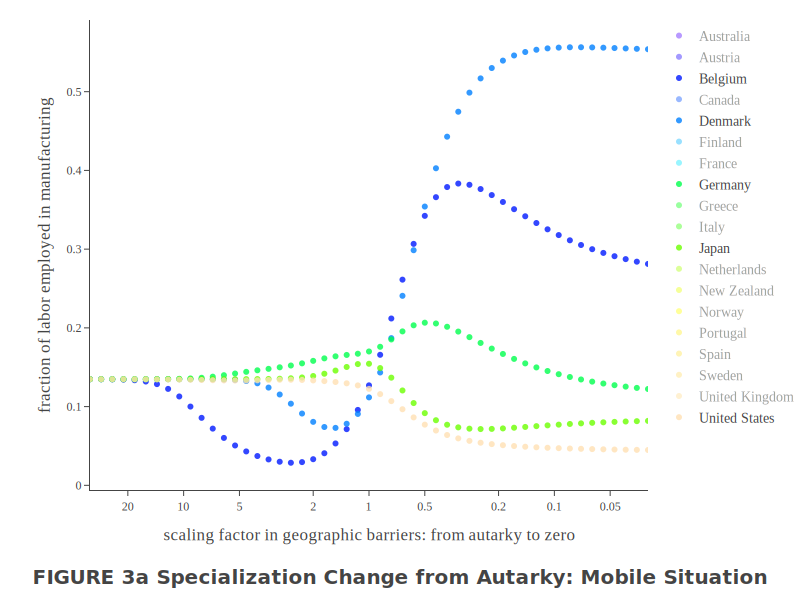
\includegraphics[width=1\linewidth]{Figures/Figure3} \end{center}

  现存的地理障碍处在一种中间状态,地理因素和技术因素共同决定着比较优势和专业化。反事实模拟的结果显示,地理障碍从目前水平下降将使技术因素变得更为重要,从而削弱大国的优势。

\hypertarget{ux5916ux56fdux6280ux672fux7684ux6ea2ux51faux6548ux5e94}{%
\subsection{外国技术的溢出效应}\label{ux5916ux56fdux6280ux672fux7684ux6ea2ux51faux6548ux5e94}}

  在现有的地理障碍水平下,一国的技术进步可以通过贸易使全世界的福利改善,该这个改善的国别分布是什么?我们先后令美国和德国的技术提高20\%,来观察标准化的各国福利变化幅度\footnote{各国福利改善的百分比除以技术进步国的福利改善百分比} 。表11显示了反事实模拟的结果。

\begin{center}\includegraphics[width=1\linewidth]{Figures/Table11} \end{center}

  当劳动力可跨部门流动时,由\eqref{eq:31}知福利只与价格有关,因为各国都享受到了价格更低的制造业产品,故各国福利普遍改善。当劳动力不可跨部门流动时,他国福利同时还受到负收入效应的影响(因为制造业工资下降)。若一国不能降低其制造业就业规模,则该国总体福利常常会下降------日本和德国是典型。

  离技术水平提高的国家越近和规模越小的国家,其福利改善的幅度越大。日本距离技术改进国既远,本身规模又大,从美国或德国的技术进步中得到的好处是最少的。

  综上,充分享受他国技术进步的溢出效应需要两个条件:(1)距离技术进步源头足够近;(2)能够将劳动力向非制造业转移。

\hypertarget{ux524aux51cfux5173ux7a0e}{%
\subsection{削减关税}\label{ux524aux51cfux5173ux7a0e}}

  我们的框架很容易结合关税收益。设进口国 \(n\) 在 \(i\) 国商品到岸价格的基础上征收从价税,税率为 \(t_{ni}\)。于是地理障碍可以拆分成自然地理障碍和关税两部分:\(d_{n i}=\left(1+t_{n i}\right) d_{n i}^{*}\)。则关税收益为:

\[
T R_{n}=\sum_{i \neq n} \frac{t_{n i}}{1+t_{n i}} X_{n i}
\]

  以所有国家对所有进口商品征收统一的5\%关税为基准,进行三种情境的反事实模拟:

\begin{enumerate}
\def\labelenumi{\arabic{enumi}.}
\item
  所有国家移除关税。劳动力可以跨部门流动时,所有国家的福利增加,且大于劳动力不可流动的情境。
\item
  美国单边移除关税。其他国家都有正的福利效应,而美国福利降低,其中加拿大的福利正效应最大。在劳动力流动情境下,其他所有国家的福利收益等于或大于美国的福利损失。这一结论说明了多边协调自由贸易的重要性。
\item
  欧洲共同体(EC)内部互相移除关税。表12表明,福利分配与劳动力是否可以跨部门流动密切相关。如第二列显示的,在劳动力不可流动时,主要的受害者是距离 EC 比较近的非 EC 成员国,它们的制造业工资下降了。在劳动力可以流动时,第一列显示,受害者是北方的 EC 国家(比利时、荷兰、丹麦、德国、英国)。这种情境下,非 EC 成员国可以通过将劳动力转移到非制造业来规避制造业工资的下降。北方 EC 国家将进口来源从非成员国转向南方 EC 国家。第三、四列表明,市场一体化使得成员国之间的贸易大量增加。而且在劳动力流动情形下,因投入品价格下降获得了一定的成本优势,EC 国家对非 EC 国家的出口通常也扩大了。
\end{enumerate}

\begin{center}\includegraphics[width=1\linewidth]{Figures/Table12} \end{center}

\hypertarget{ux7ed3ux8bba}{%
\section{结论}\label{ux7ed3ux8bba}}

  比较优势可以通过贸易创造潜在收益。然而,这些潜在收益的实现会受到地理障碍的削弱。我们的李嘉图模型可以非常简洁地捕捉这两种力量。该模型将双边贸易与技术和地理参数联系起来,我们使用了贸易流、价格和地理数据估计模型中的参数。

  尽管引力模型的文献已经认识到了地理障碍在减少贸易量中的重要性,但国际贸易的传统模型通常忽略了这些障碍。例外情况是,阿明顿假设或垄断竞争模型,这些设定通过产品差异化预先决定了专业化模式。相反,我们的框架允许地理障碍和技术共同决定专业化。它还将贸易流量与地理壁垒产生的对一价定律的偏离联系起来。

  \bibliography{mybib.bib}

\end{document}
